\documentclass[10pt]{article}
\usepackage{tabularx}
\usepackage{wrapfig}
\usepackage{parcolumns}
\usepackage{hyperref}
\usepackage{graphicx}
\usepackage{hyperref}
\usepackage{xcolor}
\usepackage{fancyhdr}
\usepackage{geometry}
\geometry{a4paper, margin=1in}

\pagestyle{fancy}
\fancyhf{}
\fancyhead[L]{Cornell Blockchain Club}
\fancyhead[C]{Monthly Newsletter}
\fancyhead[R]{June 2024}

\begin{document}

\begin{center}
    \includegraphics[width=0.3\textwidth]{logo.jpg} \\ % Add the path to your logo file
    \huge \textbf{Cornell Blockchain Club End of Year Newsletter} \\
    \large \textbf{Connecting Alumni and Current Members} \\
    \large \textbf{June 2024}
\end{center}

\vspace{1cm}

\section*{Introduction to the Newsletter Iniciative} 
\textit{Welcome to the 1st edition of the Cornell Blockchain Club Newsletter! As we wrap up the 2023-2024 academic year, we are happy to announce the launch of a monthly newsletter for both alumni and current members. This newsletter aims to keep our alumni and current members informed and connected. Your support and engagement are crucial for our ongoing success. We hope that you enjoy reading about our latest updates and accomplishments!}
\\
\textit{- Diego Fernandez}


\section*{Club Highlights}
\subsection*{Graduating Members}
As another academic year draws to a close, we proudly celebrate the achievements and contributions of our graduating members. Their dedication, innovation, and leadership have significantly enriched the Cornell Blockchain Club. We wish them all the best as they embark on their next adventures in the blockchain industry and beyond. 

\begin{parcolumns}[colwidths={1=0.45\textwidth, 2=0.45\textwidth}]{2}
    \colchunk{
        \begin{center}
            \includegraphics[width=0.2\textwidth]{Advay Koranne.jpeg} 
        \end{center}
        \subsubsection*{Advay Koranne (B.S. Computer Science and Mathematics)}
        \noindent
        Advay joined the club as a freshman in 2021. Throughout his time at CBC he has fulfilled roles ranging from teaching CS 1998 to club president. After graduation Advay will be joining Blackrock as a quant risk analyst.
    }
    \colchunk{
        \begin{center}
            \includegraphics[width=0.2\textwidth]{Diego Fernandez.jpeg} 
        \end{center}
        \subsubsection*{Diego Fernandez (B.S. Computer Science) with minor in ORIE}
        \noindent
        Diego joined the club as sophomore in 2021. For the past few years Diego has worked on arbitrage trading bots as well as participating in several trading competitions on behalf of the Trading Subteam which he led during the Fall of 2023. This past semester, Diego has been teaching the new member education course. After graduation Diego will be joining Goldman Sachs' institutional trading team.  
    }
\end{parcolumns}

\begin{parcolumns}[colwidths={1=0.45\textwidth, 2=0.45\textwidth}]{2}
    \colchunk{
        \begin{center}
            \includegraphics[width=0.2\textwidth]{Rodrigo Villar.jpeg} 
        \end{center}
        \subsubsection*{Rodrigo Villar (B.A. Computer Science and Mathematics)}
        \noindent
        Rodrigo joined Cornell Blockchain as a sophomore in fall 2021; initially starting out as a member of the then-Research and Development subteam, Rodrigo eventually rose to the position of Head of Engineering. Throughout his time in the club, Rodrigo worked on subjects ranging from arbitrage on DeFi exchanges to implementations of virtual machines. In addition to these projects, Rodrigo was responsible for the creation of CS4998: Blockchain Development, the first technical for-credit blockchain course in the Ivy League which focused on writing smart contracts with Solidity. After graduation, Rodrigo will be joining Ava Labs as a Developer Relations Engineer, where he will be working on building custom VMs using Avalanche’s HyperSDK framework.
        \noindent
    }
    \colchunk{
        \begin{center}
            \includegraphics[width=0.2\textwidth]{Daniel Mistrik.jpeg} 
        \end{center}
        \subsubsection*{Daniel Mistrik (B.A. Computer Science and Mathematics)}
        \noindent
        Daniel joined the club as a freshman in 2021. Throughout his time at CBC he has fulfilled roles ranging from teaching CS 1998 to head of trading. After graduation Daniel will be joining IMC as a software developer in Chicago.
        \noindent
    }
\end{parcolumns}


\begin{parcolumns}[colwidths={1=0.45\textwidth, 2=0.45\textwidth}]{2}
    \colchunk{
        \begin{center}
            \includegraphics[width=0.2\textwidth]{Spencer Kane.jpeg} 
        \end{center}
        \subsubsection*{Spencer Kane (B.S. Information Science)}
        \noindent
        Spencer joined the club as a sophomore in 2022. Throughout his time in Cornell Blockchain he started the consulting arm, helped to teach CS 1998, helped plan the 2023 conference, and served as Vice President. After graduation, Spencer will be looking for roles in finance and blockchain.
    }
    \colchunk{
        \begin{center}
            \includegraphics[width=0.2\textwidth]{Emir Polat.jpeg} 
        \end{center}
        \subsubsection*{Emir Polat (B.S. Computer Science)}
        \noindent
        Emir joined the club his junior spring semester and has been involved in . After graduation Emir will be working at Avalanche. 
\noindent
    }
\end{parcolumns}

\vspace{1cm}

\subsection*{Cornell Blockchain Accelerator}
    The Cornell Blockchain Accelerator, led by Yousuf Qaum, is dedicated to fostering innovation and growth in the blockchain sector. 
    \vspace{0.2cm}
    \noindent
    To date, the program has completed three cohorts, encompassing 12 startups that have collectively raised over \$2.4 million. Now held annually during the spring semester, the accelerator offers technical workshops, business and strategy lectures, with flagship events including mid-semester pitch deck reviews and a Demo Day at the Cornell Blockchain Conference.
    
    \vspace{0.2cm}
    \noindent
    As we prepare for our next launch in the spring of 2025, the accelerator is seeking assistance with mentorship, providing startup credits, and other support typical of accelerator programs. Please reach out to \textcolor{blue}{yaq2@cornell.edu} if you have any information or leads to help us run the program.
    \vspace{0.2cm}
    \begin{parcolumns}{4}
        \colchunk{
            \href{https://hvaxapp.com}{Event Horizon} 
        }
        \colchunk{
            \href{https://twitter.com/Manda_Labs}{Manda Labs}
        }
        \colchunk{
            \href{}{DividX}
        }
        \colchunk{
            \href{}{Souvenir}
        }
    \end{parcolumns}
    \vspace{0.2cm}
    \begin{parcolumns}{4}
        \colchunk{
            \href{https://meritic.xyz/}{Meritic} 
        }
        \colchunk{
            \href{https://www.nau.finance/}{Nau Finance}
        }
        \colchunk{
            \href{https://www.revamia.com/}{Revamia}
        }
        \colchunk{
            \href{}{SGX}
        }
    \end{parcolumns} 
    \vspace{0.2cm}
        \begin{parcolumns}{4}
        \colchunk{
            \href{https://getpolyplatform.com/}{PolyPlatform} 
        }
        \colchunk{
            \href{}{MintMatch}
        }
        \colchunk{
            \href{https://github.com/orbit-cdp}{Orbit}
        }
        \colchunk{
            \href{https://gradientfi.com/}{GradientFi}
        }
    \end{parcolumns}
    

\vspace{1cm}
\subsection*{0xCastle}
\begin{center}
    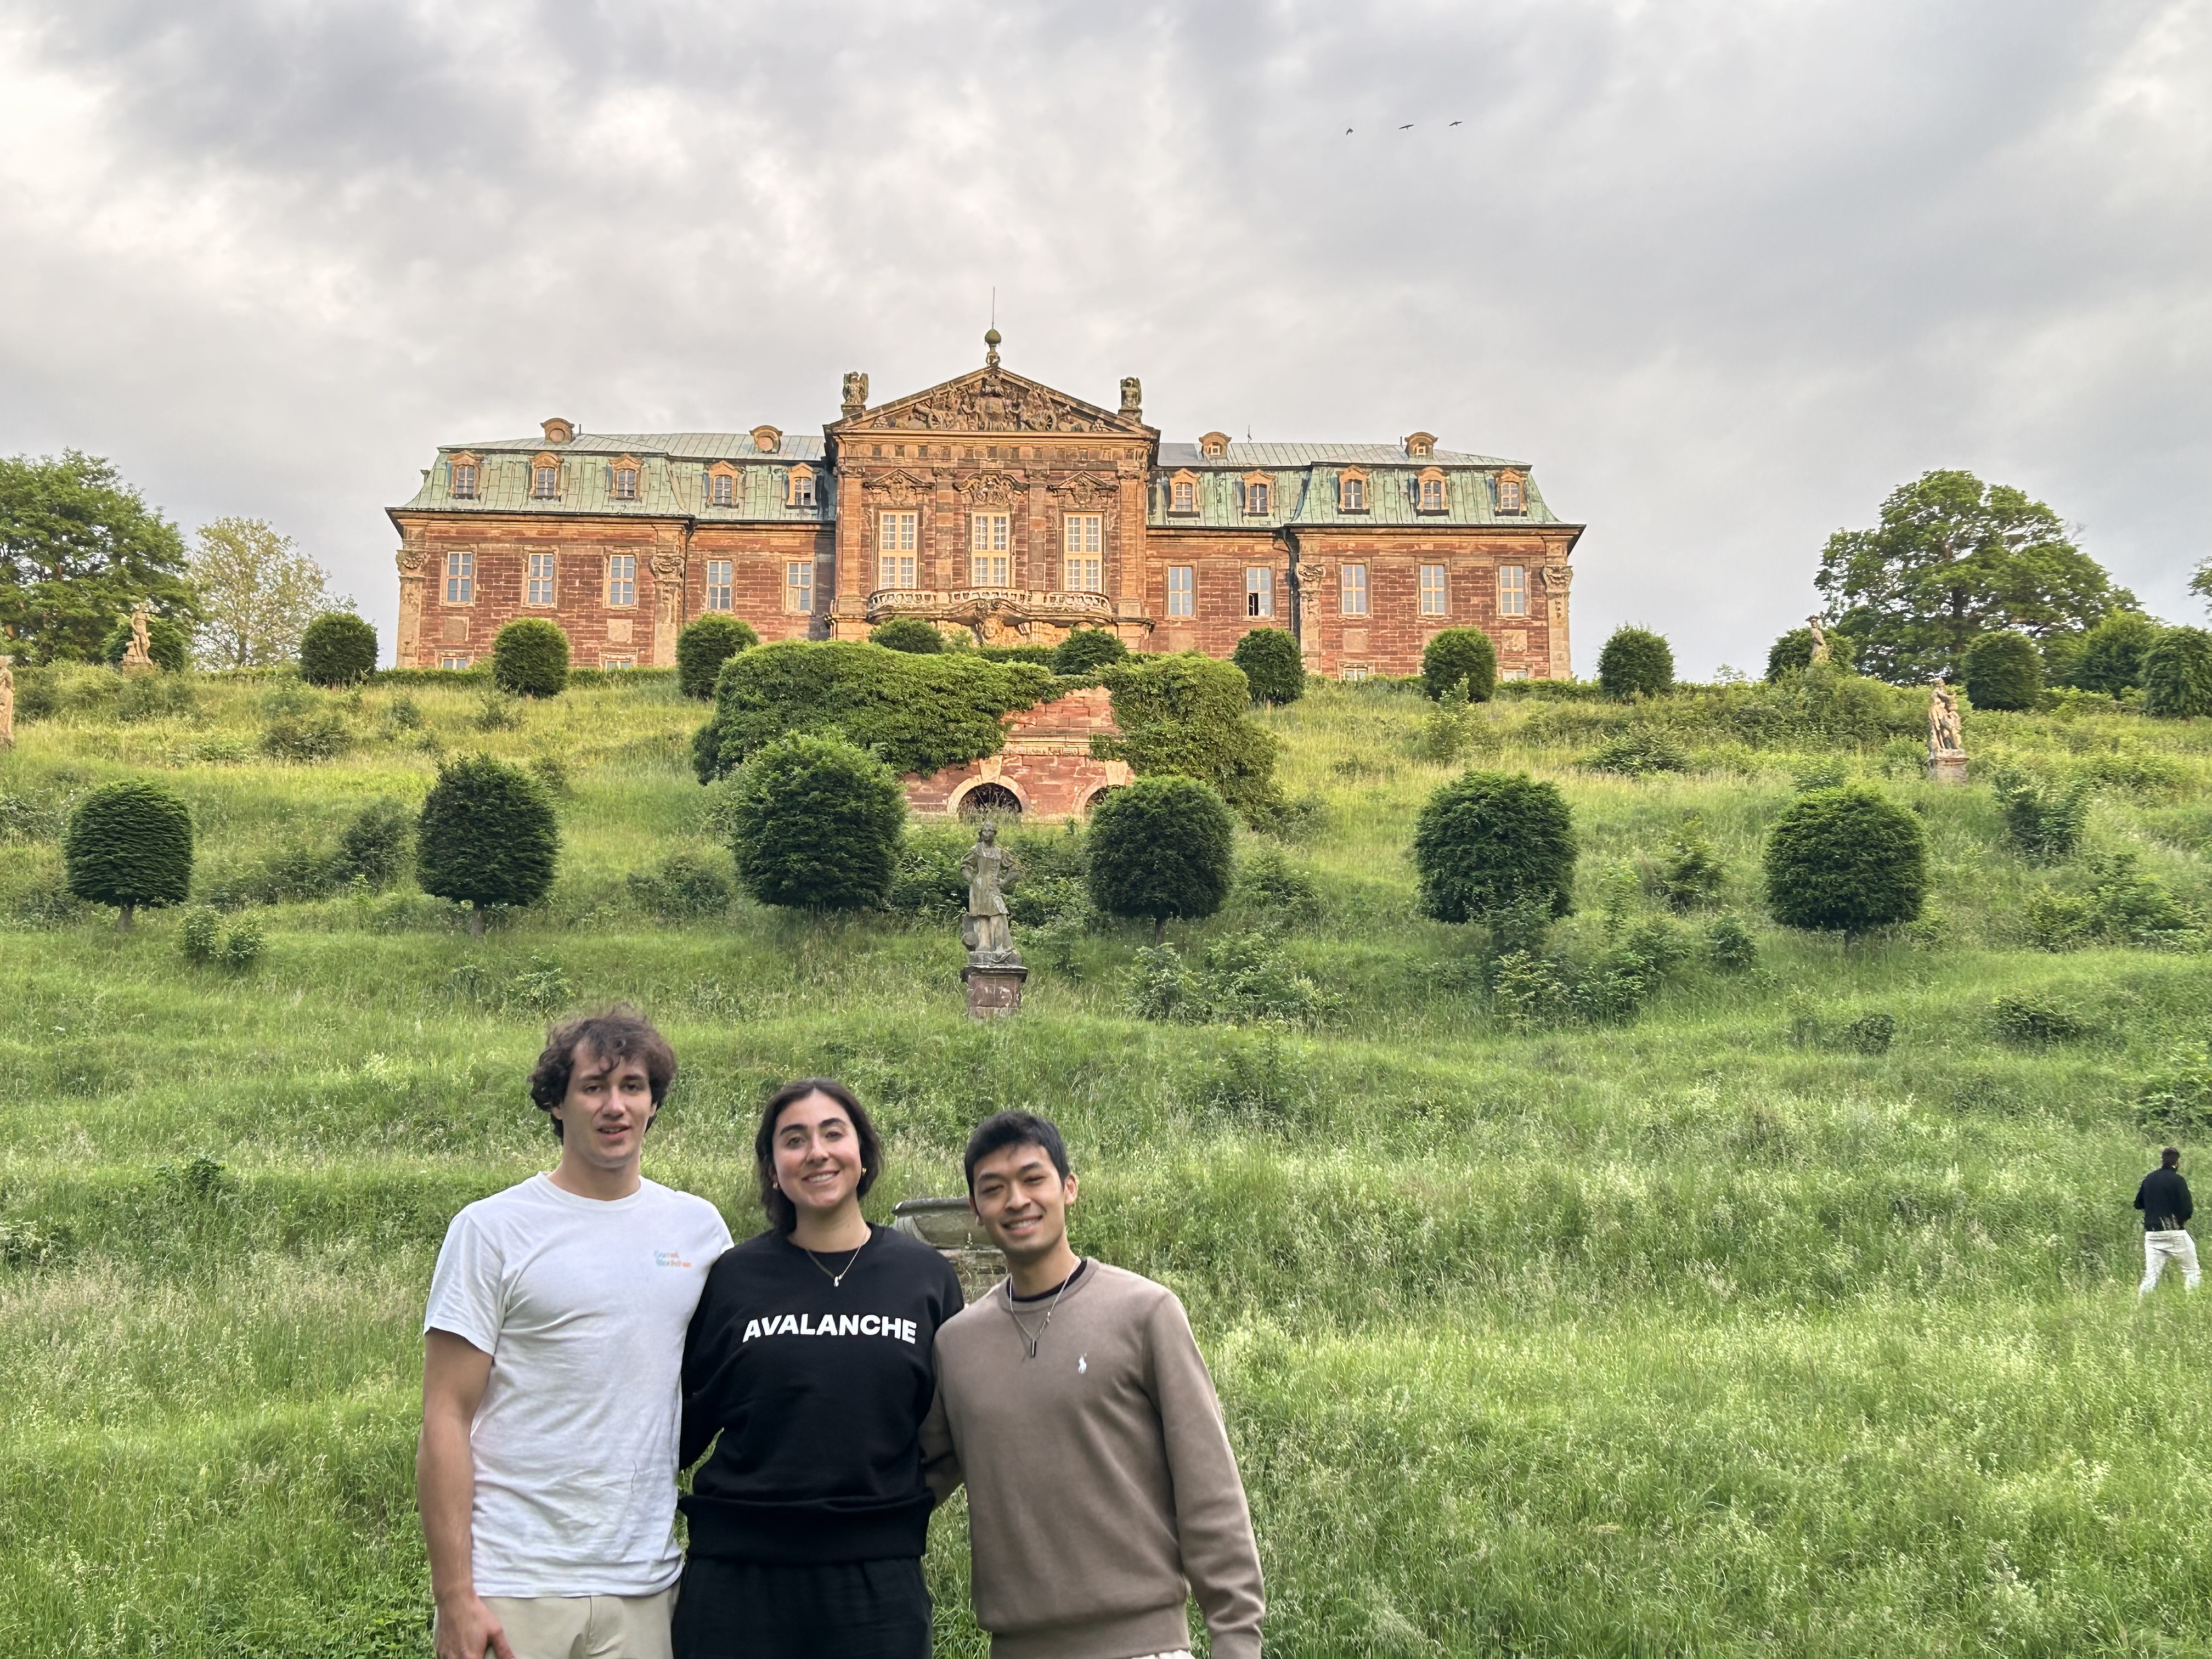
\includegraphics[width=0.45\textwidth]{0xCastle Team Picture.jpg}
\end{center}
\noindent
This past week Leah Valente, Alex Tang and Diego Fernandez attended the annual 0xCastle event hosted by TUM Blockchain Club near Leipzig, Germany. Throughout the 5 week retreat, our members attended talks on the topics of Cryptography, Rollups, and MEVs.





\section*{Sub-Team Reports}
\begin{parcolumns}{3}
    \colchunk{
        \begin{center}
            \includegraphics[width=0.2\textwidth]{Edu Logo.png}
        \end{center}
        \subsection*{Education Team}
            \textbf{CS-1998:} 
            This semester's edition of the Intro to Blockchain class was taught by Ilan Klimberg.
            Throughout the semester, Ilan remained true to his vision of providing an accessible course to all individuals by reducing the technical knowledge encouraged in prior semesters and expanding the scope
            of the concepts covered such as a brief introduction to TradFi and DeFi by guest lecturer Diego Fernandez.
            The class also gained first hand insight into the developing industry
            through guest lectures by industry leader and club alumni Nick Stamm!
            Ilan plans to add more guest lecturers in the future.  Additionally, the class will include labs where students will make wallets together, mint NFTs, and present on cryptocurrencies they believe will go up based on metrics learned in class.
            \noindent
            \\\\
            \textbf{CS-4998:} 
            This brand new course taught by Rodrigo Villar (head of reasearch at CBC) introduced students to the Solidity smart contract language as well as development tools such as Hardhat, Infura, Metamask. This 12 week course was taught using the following \href{https://cs4998.cornellblockchain.org}{textbook}, fully developed by Rodrigo Villar.
    }
    \colchunk{
        \begin{center}
            \includegraphics[width=0.2\textwidth]{Gov Logo.png}
        \end{center}
        \subsection*{Governance Team}
            Governance this semester has been voting on Arbitrum, with proposals so far including protocol improvements, budget adjustments, smart contract optimizations, and initiatives involving the network's security and scalability. Some more specific ones are the Stable Treasury Endowment Program, which creates a sustainable endowment for financial stability, and LTIPP, which solves the problem of burdens on delegates by creating alternate incentives with a council approach. We've also recently gained delegation in Optimism governance, where we are becoming active and voting on new proposals there as well. There are many different proposals across both platforms, but we vote every week after doing adequate research.
    }
    \colchunk{
        \begin{center}
            \includegraphics[width=0.2\textwidth]{Eng Logo.png}
        \end{center}
        \subsection*{Engineering Team}
            The eng...
    }
\end{parcolumns}

\begin{parcolumns}{3}
    \colchunk{
        \begin{center}
            \includegraphics[width=0.2\textwidth]{Cons Logo.png}
        \end{center}
        \subsection*{Consulting Team}
        This semester, the Consulting Team engaged in two notable activities. First, we partnered with AthenaDAO, a DAO focused on funding women’s health initiatives. We researched proposed Web3 data storage solutions to improve data security, user accessibility, and scalability for various organizational needs. Second, we were one of fifteen clubs at Cornell selected to participate in the Deloitte Undergraduate Case Competition. Our team analyzed a business problem and presented our solution to consultants at Deloitte.
    }
    \colchunk{
        
    }
    \colchunk{
       
    }
\end{parcolumns}


\vspace{1cm}

\begin{itemize}
    \item \textbf{Mastering Ethereum Book:} A comprehensive resource developed by our members.
    \item \textbf{Light EVM:} A lightweight Ethereum Virtual Machine implementation by Rodrigo Villar.
    \item \textbf{NFT Utility Standard:} An innovative standard developed by Prawira Pikanto.
\end{itemize}

\vspace{1cm}

\section*{Upcoming Events}
\textbf{Cornell Blockchain Club Conference 2024:}
\begin{itemize}
    \item \textbf{Date:} April 15-17, 2024
    \item \textbf{Location:} NYC
    \item \textbf{Description:} Join us for a series of talks, panels, and networking events with leaders from academia and the blockchain industry.
\end{itemize}

\textbf{Workshops and Seminars:}
Stay tuned for upcoming workshops on smart contract development and blockchain security.

\vspace{1cm}

\section*{Job and Internship Opportunities}


\vspace{1cm}

\section*{Get Involved}
\textbf{Mentorship Program:} Alumni interested in mentoring current members can sign up [here].
\noindent
\textbf{Speaking Opportunities:} We are looking for alumni to speak at our events. Contact us if you are interested.

\textbf{Donations:} Your donations help us fund projects and events. Donate [here].

\vspace{1cm}

\section*{Contact Information}
\textbf{Email:} \href{mailto:contact@cornellblockchainclub.com}{contact@cornellblockchainclub.com} \\
\textbf{Website:} \href{https://www.cornellblockchainclub.com}{www.cornellblockchainclub.com} \\
\textbf{Social Media:} [List of social media handles]

\end{document}
